\documentclass{standalone}
\usepackage{tikz}
\usetikzlibrary{positioning}
\usetikzlibrary {shapes.geometric}
\usetikzlibrary {backgrounds}
\usepackage[nomessages]{fp}

\tikzstyle{lOneBlock} = [circle, draw, fill=lightgray, inner sep=2]
\tikzstyle{lOneTx} = [rectangle, minimum width=1cm, minimum height = 0.1cm, inner sep=0, outer sep=0]
\tikzstyle{lTwoTx} = [rectangle, blue, minimum width=0.4cm, minimum height = 0.1cm, inner sep=0, outer sep=0]
\tikzstyle{background rectangle} = [fill=white]


\newcommand{\timeline}{
    \node (t0) at (0,0) {};
    \node (tEnd) at (10,0) {};
    \draw (t0) [->, thick]  -- (tEnd);
    \foreach \idx in {0,...,2}{
        \node (lOneBlock\idx) [lOneBlock] at (1 + \idx * 4, 0) {};
    };
}

\newcommand{\lOneTransactions}{
    \foreach \blockIdx in {0,...,2}{
        \node (txPos) at (0, 1) {};
        \foreach \txIdx in {0,...,5} {
            \node[draw, lOneTx, anchor=north] (tx-\blockIdx-\txIdx) at (lOneBlock\blockIdx |- txPos) {};
            \node (txPos) at (tx-\blockIdx-\txIdx.south) {};
        }
    };
    \node[yshift=0.1cm, anchor=south] at (tx-0-0.north) {\tiny \texttt{Block x-2}};
    \node[yshift=0.1cm, anchor=south] at (tx-1-0.north) {\tiny \texttt{Block x-1}};
    \node[yshift=0.1cm, anchor=south] at (tx-2-0.north) {\tiny \texttt{Block x}};
}

\begin{document}

% Introduce L1 chain
\ifnum \sourceNo = 0
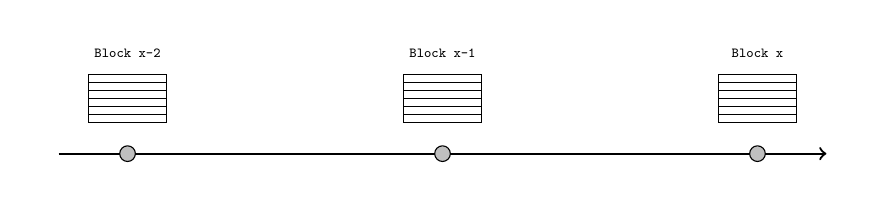
\begin{tikzpicture}[framed]
    \timeline
    \lOneTransactions
\end{tikzpicture}
\fi

% Instead of passing parameters to the diagram commands, define them as variables
% This makes it easier to reuse variables between different diagrams and also makes the diagram commands more readable
\newcommand{\anchorBlockNum}{1}
\newcommand{\numLTwoBlocks}{6}
\newcommand{\pubTx}{tx-2-3}
\newcommand{\anchorBlock}{lOneBlock\anchorBlockNum}

\newcommand{\lTwoTransactions}{
    \node[yshift=-0.3cm, xshift=0.5cm] (blockPos) at (\anchorBlock) {};
    \foreach \idx in {0,...,\numLTwoBlocks}{
        \node (lTwoBlock\idx)  at (blockPos) {};
        \node (blockPos) at (blockPos)[xshift=0.5cm] {};
    };

    \foreach \blockIdx in {0,...,\numLTwoBlocks} {
        \node (txPos) at (lTwoBlock\blockIdx) {};
        \foreach \txIdx in {0,...,4}{
            \node[draw, lTwoTx, anchor=north] (l2Tx-\blockIdx-\txIdx) at (txPos) {};
            \node (txPos) at (l2Tx-\blockIdx-\txIdx.south) {};
        }
    }
}

\newcommand{\publication}{
    \node[draw, lOneTx, fill=blue] at (\pubTx) {};
    \node[xshift=-0.1cm, yshift=0.1cm] (topLeft) at (l2Tx-0-0.north west) {};
    \node[xshift=0.1cm, yshift=-0.1cm] (bottomRight) at (l2Tx-\numLTwoBlocks-4.south east) {};
    \draw[very thin] (topLeft) rectangle (bottomRight) {};
    \draw[very thin] (topLeft) -- (\pubTx.north west);
    \draw[very thin] (bottomRight |- topLeft) -- (\pubTx.north east);
}

% Introduce L2 chain
\ifnum \sourceNo = 1
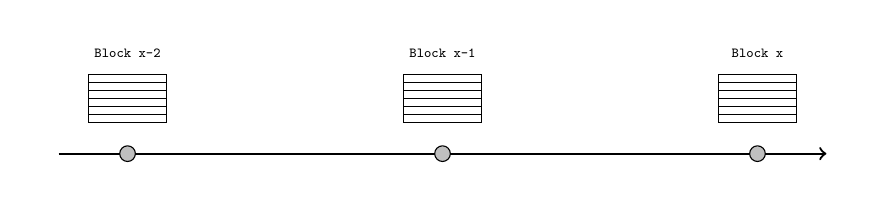
\begin{tikzpicture}[framed]
    \timeline
    \lOneTransactions
    \lTwoTransactions
    \publication
\end{tikzpicture}
\fi

% L2 publications may span multiple L1 slots
\renewcommand{\anchorBlockNum}{0}
\renewcommand{\numLTwoBlocks}{13}

\ifnum \sourceNo = 2
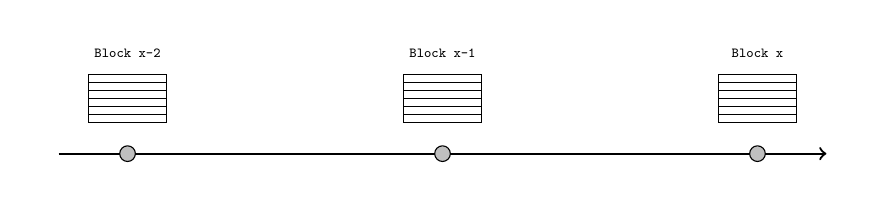
\begin{tikzpicture}[framed]
    \timeline
    \lOneTransactions
    \lTwoTransactions
    \publication
\end{tikzpicture}
\fi

\newcommand{\snapshotAt}[1]{
    \node (top) at (#1, 1.5) {};
    \node (bottom) at (#1, -1) {};

    \fill [fill=white, opacity=0.7] (top) rectangle (tEnd |- bottom);
    \clip (t0 |- top) rectangle (bottom);
}

\newcommand{\injectAnchor}{
    \node[draw, lOneBlock, fill=magenta] at (\anchorBlock) {};
    \node[draw, lTwoTx, fill=magenta, minimum width=0.1cm, anchor=west] at (l2Tx-0-0.west) {};
    \draw[->, magenta] (\anchorBlock.south) to[bend right] (l2Tx-0-0.west);
}

% Snapshot after L2 transaction
\ifnum \sourceNo = 3
\begin{tikzpicture}[framed]
    \timeline

    \snapshotAt{4.25}
    
    \lOneTransactions
    \lTwoTransactions
    \injectAnchor

    \node[draw, lOneTx, fill=teal] at (tx-0-4) {};
    \node[draw, lTwoTx, fill=green] at (l2Tx-1-2) {};
\end{tikzpicture}
\fi

\newcommand{\validateAnchor}{
    \node[draw, lOneTx, fill=magenta, minimum width=0.1cm, anchor=west] at (\pubTx.west) {};
    \draw[->, magenta] (\anchorBlock.north east) to[bend left] (\pubTx.west);
}

% Anchor block hash is validated
\ifnum \sourceNo = 4
\begin{tikzpicture}[framed]
    \timeline

    \lOneTransactions
    \lTwoTransactions
    \publication
    \injectAnchor
    \validateAnchor

    \node[draw, lOneTx, fill=teal] at (tx-0-4) {};
    \node[draw, lTwoTx, fill=green] at (l2Tx-1-2) {};

\end{tikzpicture}
\fi

% Anchor block hash is validated
\ifnum \sourceNo = 5
\begin{tikzpicture}[framed]
    \timeline

    \lOneTransactions
    \lTwoTransactions
    \publication
    
    \node[draw, lOneTx, fill=orange] at (tx-2-1) {};
    \node[draw, lTwoTx, fill=orange, minimum width=0.1cm, anchor=west] (assertion) at (l2Tx-9-0.west) {};
    \draw[->, orange] (tx-2-1.west) to[bend right] (assertion.north);

    \node[draw, lTwoTx, fill=green] at (l2Tx-9-2) {};
\end{tikzpicture}
\fi

\end{document}



        